% --------------------------------------------------------------
% This is all preamble stuff that you don't have to worry about.
% Head down to where it says "Start here"
% --------------------------------------------------------------
 
\documentclass[10pt]{article}

 \usepackage{tikz}
\usepackage[margin=1in]{geometry} 
\usepackage{amsmath,amsthm,amssymb}
 
\newcommand{\N}{\mathbb{N}}
\newcommand{\Z}{\mathbb{Z}}
 
\newenvironment{theorem}[2][Theorem]{\begin{trivlist}
\item[\hskip \labelsep {\bfseries #1}\hskip \labelsep {\bfseries #2.}]}{\end{trivlist}}
\newenvironment{lemma}[2][Lemma]{\begin{trivlist}
\item[\hskip \labelsep {\bfseries #1}\hskip \labelsep {\bfseries #2.}]}{\end{trivlist}}
\newenvironment{exercise}[2][Exercise]{\begin{trivlist}
\item[\hskip \labelsep {\bfseries #1}\hskip \labelsep {\bfseries #2.}]}{\end{trivlist}}
\newenvironment{reflection}[2][Reflection]{\begin{trivlist}
\item[\hskip \labelsep {\bfseries #1}\hskip \labelsep {\bfseries #2.}]}{\end{trivlist}}
\newenvironment{proposition}[2][Proposition]{\begin{trivlist}
\item[\hskip \labelsep {\bfseries #1}\hskip \labelsep {\bfseries #2.}]}{\end{trivlist}}
\newenvironment{corollary}[2][Corollary]{\begin{trivlist}
\item[\hskip \labelsep {\bfseries #1}\hskip \labelsep {\bfseries #2.}]}{\end{trivlist}}
\newenvironment{solution}[2][Solution]{\begin{trivlist}
\item[\hskip \labelsep {\bfseries #1}\hskip \labelsep {\bfseries #2.}]}{\end{trivlist}}

\theoremstyle{definition}
\newtheorem*{defn*}{Definition}
\newtheorem{conj}{Conjecture}[section]
\newtheorem{exmp}{Example}[section]
\newtheorem{bas}{Basis}[section]

 
\begin{document}
 
% --------------------------------------------------------------
%                         Start here
% --------------------------------------------------------------
 
%\renewcommand{\qedsymbol}{\filledbox}
 
\title{CS310: Homework 7}%replace X with the appropriate number
\author{Scott Fenton\\ %replace with your name
} %if necessary, replace with your course title
 
\maketitle
\begin{exercise}{(1)}
Write the vertices in the order encountered during a BFS, starting from vertex A. Break ties
by alphabetical order.\\
\\
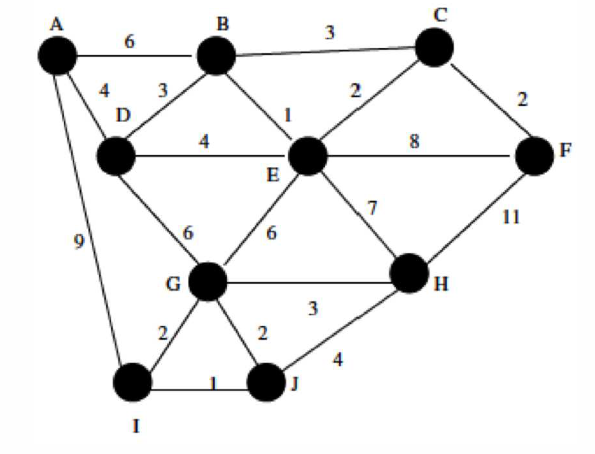
\includegraphics[width=100mm,scale=0.3]{p1.PNG}\\
\end{exercise}

\begin{solution}{(1)}
Output: A-B-D-I-C-E-G-J-F-H	\\
Working node A. Enqueue B. Queue[B]\\
Working node A. Enqueue D. Queue[D B]\\
Working node A. Enqueue I. Queue[I D B]\\
Dequeue B.\\
Working node B. Enqueue C. Queue[C I D]\\
Working node B. Enqueue E. Queue[E C I D]\\
Dequeue D.\\
Working node D. Enqueue G. Queue[G E C I]\\
Dequeue I.\\
Working node I. Enqueue J. Queue[J G E C]\\
Dequeue C.\\
Working node C. Enqueue F. Queue[F J G E]\\
Dequeue E.\\
Working node G. Enqueue H. Queue[H F J G]\\
\end{solution}


\begin{exercise}{(2)} %You can use theorem, proposition, exercise, or reflection here.  Modify x.yz to be whatever number you are proving
Do the same with a DFS, and break ties by reverse alphabetical order.\\
\end{exercise}
 
\begin{solution}{(2)}
Output: A-I-J-H-G-E-F-C-B-D\\
Push A.\\
Working node A. Push I. Stack[A I]\\
Working node I. Push J. Stack[A I J]\\
Working node J. Push H. Stack[A I J H]\\
Working node H. Push G. Stack[A I J H G]\\
Working node G. Push E. Stack[A I J H G E]\\
Working node E. Push F. Stack[A I J H G E F]\\
Working node F. Push C. Stack[A I J H G E F C]\\
Working node C. Push B. Stack[A I J H G E F C B]\\
Working node B. Push D. Stack[A I J H G E F C B D]\\
\end{solution}


\begin{exercise}{(3)}
Do a topological sort of the following graph with the edge (H,G) removed.\\
\\
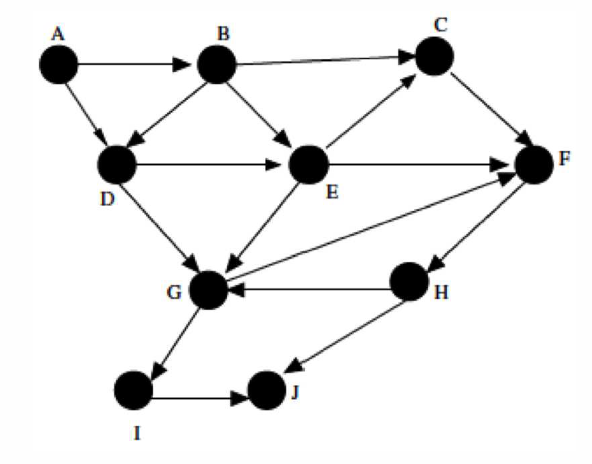
\includegraphics[width=80mm,scale=0.2]{p3.PNG}\\
\end{exercise}

\begin{solution}{(3)}
The Graph with edge (H,G) removed:\\
\\
\\Topological sort: A-B-D-E-G-I-C-F-H-J\\
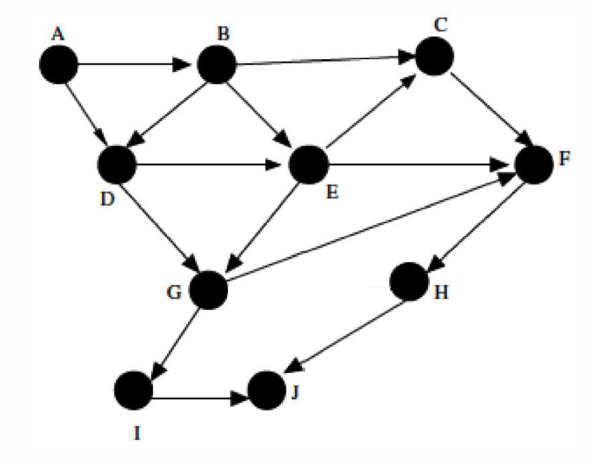
\includegraphics[width=80mm,scale=0.2]{p3impr.PNG}\\



\end{solution}


\begin{exercise}{(4)}
Is the topological sort you found in Problem 3 a unique one? If yes, say so – if no, give another
topological sort.\\
\end{exercise}

\begin{solution}{(4)}
No, an alternate topological sort is:
A-B-D-E-C-G-I-F-H-J
\end{solution}
% --------------------------------------------------------------
%     You don't have to mess with anything below this line.
% --------------------------------------------------------------
 
\end{document}